\chapter{Results and Discussion}\label{chap: results}

We start by presenting an elementary approach to this research problem. Then we move on to the comparison of results (judging mainly by the accuracy). The results are presented using the neural network model and it is compared with baseline methods. The comparison is divided into two parts (i) first, predicting the disease terms and (ii) second, predicting the super class of the disease terms.

The dataset was tested with three types of problem transformations (refer Section~\ref{MLtranform}): (i) Binary Relevance, (ii) Label Powerset and (iii) Classifier Chains. The problem transformations were used from scikit-multilearn that is a library specific to multi-label classification built on top of the well-known scikit-learn.~\cite{2017arXiv171100046S}. The classifiers that were tested using these transformations were 
\begin{itemize}
    \item Multi-layer Perceptron classifier (MLP classifier) 
    \item Multi-label k Nearest Neighbour (MLkNN) 
    \item Random Forest Classifier 
    \item Decision Trees Classifier 
\end{itemize}
For each combination the evaluation metrics used were: accuracy, hamming loss, weighted F1 score and weighted precision score. The classifiers used and the metrics were calculated using scikit-learn~\cite{scikit-learn}. 

For the neural network approach we utilized the pretrained word embeddings - GloVe: Global Vectors for Word Representation~\cite{pennington2014glove} of length 300. For data preprocessing we used tokenizer API from Keras~\cite{chollet2015keras}. The CNN and BiLSTM architectures were used from PyTorch\footnote{\url{https://pytorch.org/}}.
For validating the results using the Neural Networks we split the data into training and validation sets. The training set is 80\% of the whole data and the validation set is the rest 20\%. A similar train-test split was done for the baseline mu;ti-label classification 80\%-20\%. The dropout rate has been kept $0.2$ in all the neural network models. 

\section{An elementary approach}
In prediction of metadata, specifically diseases - an elementary approach would be to use a vocabulary of disease names, and perform a basic search in the documents. If we have a match it can be said that a particular publication talks about `xyz' disease. This would be a direct and trivial way to approach this problem. 

In this case, since the dataset majorly uses the MeSH ontology, so all the values of disease names is downloaded\footnote{\url{http://bioportal.bioontology.org/ontologies/MESH/?p=classes&conceptid=root}}. After that, a direct matching is done using Flashtext~\cite{2017arXiv171100046S}. Firstly the downloaded diseases from the MeSH contains a lot of secondary information which is not essential, therefore columns with disease names are selected. This also includes the synonyms so that the matching is not biased for terms like `heart disease' and `cardiovascular disease'. Even after including the synonyms we could find only $44$ unique terms in the text, which is $\approx$2\% of the diseases identified disease terms.



\section{Predicting Disease Terms}
For prediction of disease terms, the unique ID (explained in Section~\ref{section:data}) were used as labels after preprocessing - removing duplicates and characters if present. 

\subsection{Baseline Multi-label Classification}
For baseline multi-label classification two type of feature extraction techniques were used: (i) TF-IDF and (ii) Bag of words representation (BoW). The results for these two techniques are presented in Tables~\ref{tab:resultdiseasetfidf} and~\ref{tab:resultdiseasecount}. For both the techniques the maximum feature length is kept 200. It can be seen that the MLP Classifier performs the best in both the techniques of feature extraction. 

There is a difference in the performance if we compare the different feature extraction methods, the TF-IDF technique performs better. The TF-IDF normalizes the outputs which is why this technique is known to perform better when comes to the feature selection, it can be observed from the results as well. 
Since dataset has a large number of diseases - $588$, and a limited number of abstracts, the accuracy of predictions is not very high. The highest accuracy that we get here is $\approx 19\%$. 

\begin{table}[!htb]
    \centering
    \resizebox{\textwidth}{!}{%
\begin{tabular}{|c|l|l|l|l|l|l|l|l|l|l|l|l|l|}
\hline
\multicolumn{1}{|l|}{\multirow{2}{*}{}}                               & \multicolumn{3}{c|}{Random forest}                                          & \multicolumn{3}{c|}{Decision Tree}                                          & \multicolumn{3}{c|}{MLPClassifier}                                          & \multicolumn{4}{c|}{MLkNN}                                                                                   \\ \cline{2-14} 
\multicolumn{1}{|l|}{}                                                & \multicolumn{1}{c|}{BR} & \multicolumn{1}{c|}{LP} & \multicolumn{1}{c|}{CC} & \multicolumn{1}{c|}{BR} & \multicolumn{1}{c|}{LP} & \multicolumn{1}{c|}{CC} & \multicolumn{1}{c|}{BR} & \multicolumn{1}{c|}{LP} & \multicolumn{1}{c|}{CC} & \multicolumn{1}{c|}{k=20} & \multicolumn{1}{c|}{k=30} & \multicolumn{1}{c|}{k=10} & \multicolumn{1}{c|}{k=5} \\ \hline
Accuracy                                                              & \textbf{0.101}          & 0.075                   & 0.088                   & 0.044                   & \textbf{0.107}          & 0.082                   & 0.170                   & \textbf{0.189}          & 0.164                   & 0.164                     & 0.138                     & \textbf{0.176}            & \textbf{0.176}           \\ \hline
hamming loss                                                          & 0.004                   & 0.007                   & 0.004                   & 0.007                   & 0.007                   & 0.007                   & 0.004                   & 0.005                   & 0.004                   & 0.004                     & 0.004                     & 0.004                     & 0.004                    \\ \hline
\begin{tabular}[c]{@{}c@{}}F1 score \\ (weighted)\end{tabular}        & 0.125                   & 0.191                   & 0.117                   & 0.259                   & 0.208                   & 0.250                   & 0.207                   & 0.233                   & 0.203                   & 0.194                     & 0.184                     & 0.238                     & 0.232                    \\ \hline
\begin{tabular}[c]{@{}c@{}}precision score \\ (weighted)\end{tabular} & 0.226                   & 0.197                   & 0.188                   & 0.264                   & 0.235                   & 0.250                   & 0.226                   & 0.250                   & 0.234                   & 0.218                     & 0.231                     & 0.258                     & 0.263                    \\ \hline
\end{tabular}%
}
    \caption{Results for Disease terms using TF-IDF feature selection}
    \label{tab:resultdiseasetfidf}
\end{table}

\begin{table}[!htb]
    \centering
    \resizebox{\textwidth}{!}{%
\begin{tabular}{|c|l|l|l|l|l|l|l|l|l|l|l|l|l|}
\hline
\multicolumn{1}{|l|}{\multirow{2}{*}{}} & \multicolumn{3}{c|}{Random forest} & \multicolumn{3}{c|}{Decision Tree} & \multicolumn{3}{c|}{MLPClassifier} & \multicolumn{4}{c|}{MLkNN} \\ \cline{2-14} 
\multicolumn{1}{|l|}{} & \multicolumn{1}{c|}{BR} & \multicolumn{1}{c|}{LP} & \multicolumn{1}{c|}{CC} & \multicolumn{1}{c|}{BR} & \multicolumn{1}{c|}{LP} & \multicolumn{1}{c|}{CC} & \multicolumn{1}{c|}{BR} & \multicolumn{1}{c|}{LP} & \multicolumn{1}{c|}{CC} & \multicolumn{1}{c|}{k=20} & \multicolumn{1}{c|}{k=30} & \multicolumn{1}{c|}{k=10} & \multicolumn{1}{c|}{k=5} \\ \hline
Accuracy & 0.088 & \textbf{0.126} & 0.088 & 0.082 & 0.094 & \textbf{0.113} & 0.132 & \textbf{0.157} & 0.126 & 0.088 & 0.088 & \textbf{0.107} & 0.082 \\ \hline
hamming loss & 0.004 & 0.006 & 0.004 & 0.008 & 0.008 & 0.008 & 0.004 & 0.005 & 0.004 & 0.004 & 0.004 & 0.004 & 0.005 \\ \hline
\begin{tabular}[c]{@{}c@{}}F1 score \\ (weighted)\end{tabular} & 0.106 & 0.160 & 0.090 & 0.256 & 0.191 & 0.257 & 0.175 & 0.217 & 0.171 & 0.098 & 0.091 & 0.128 & 0.163 \\ \hline
\begin{tabular}[c]{@{}c@{}}precision score \\ (weighted)\end{tabular} & 0.158 & 0.178 & 0.152 & 0.250 & 0.216 & 0.262 & 0.217 & 0.241 & 0.216 & 0.166 & 0.167 & 0.172 & 0.199 \\ \hline
\end{tabular}%
}
    \caption{Results for Disease terms using Bag of words feature selection}
    \label{tab:resultdiseasecount}
\end{table}

\subsection{Neural Network Method}
For the neural network method. Two models were trained - (i) BiLSTM and (ii) CNN. The embedding dimension in both cases is 300, where the input sequences are kept as 200 for which the results are discussed. The models are also retrained for a sequence length of 150 and 250 to check whether the accuracy increases or decreases. The models are trained using the Adam optimizer~\cite{kingma2014adam}. 

The results of models are presented in Table~\ref{tab:DLdiseases}. The number of epochs are kept high because of a large number of labels. Here it can be seen that the CNN outperforms all the baseline methods and the BiLSTM. Whereas the BiLSTM has a lesser accuracy than highest baseline MLP classifier. One explanation would be that since the RNN treats the input as a sequence, and its a very long sequence, as it goes ahead working on word after word, it forgets what happened in the words before. Even though we're using a bidirectional RNN, maybe the left to right forgets what happened at the start, say by the time it reaches mid sequence, and the right to left forgets what it saw in the first (rightmost) terms by the time it reaches mid sequence too. 

Whereas in CNNs, the convolution kernels are time invariant so they cannot distinguish between different parts of the sequence. As a disadvantage, they cannot easily do inferences which require using context, and need to treat the input as a sequence. However in this case, it might not be needed. Abstracts may somewhere mention a particular disease keyword  which is enough on its own to detect which class it belongs to (and this detection requires no sequential treatment of input, which is similar to `find a word').

\begin{table}[!htb]
\centering
\begin{tabular}{|l|l|l|l|}
\hline
\multicolumn{1}{|c|}{} & \multicolumn{1}{c|}{\textbf{Epochs}} & \multicolumn{1}{c|}{\textbf{\begin{tabular}[c]{@{}c@{}}Validation \\ Accuracy\end{tabular}}} & \multicolumn{1}{c|}{\textbf{\begin{tabular}[c]{@{}c@{}}Sequence\\  Length\end{tabular}}} \\ \hline
\textbf{BiLSTM} & 200 & \textit{\textbf{0.177}} & 200 \\ \hline
 & 200 & 0.168 & 150 \\ \hline
 & 200 & 0.099 & 250 \\ \hline
\textbf{CNN} & 180 & 0.31 & 200 \\ \hline
 & 180 & 0.283 & 150 \\ \hline
 & 180 & \textit{\textbf{0.335}} & 250 \\ \hline
\end{tabular}
\caption{Results for deep neural networks for predicting disease names}
\label{tab:DLdiseases}
\end{table}

\section{Predicting Super Class}
In this experiment we use the MeSH tree structure\footnote{\url{https://meshb.nlm.nih.gov/treeView}} to map the annotated disease names to their super classes shown in Figure~\ref{fig:meshsuperclass}. 
\begin{figure}[!htb]
    \centering
    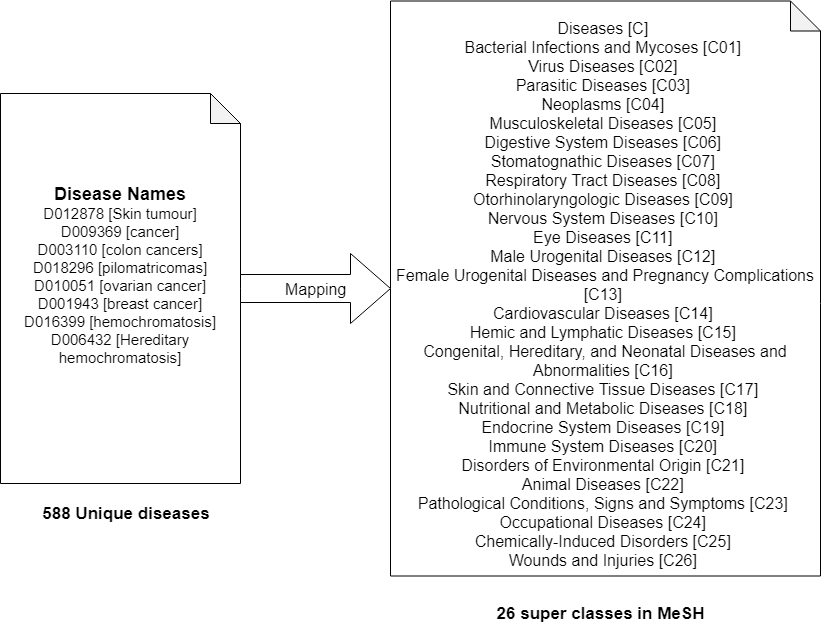
\includegraphics[scale=0.45]{Figures/NN_prediction.png}
    \caption{Mapping super classes in MeSH}
    \label{fig:meshsuperclass}
\end{figure}
To do so we use the unique ID of the disease terms as explained in Section~\ref{section:data} to do a SPARQL query to map these terms (refer Listing~\ref{superclassquery}). The motivation behind this experiment setup is to reduce the number of labels that the method had to predict. This is done for each abstract, then these new super classes are used as target labels. 

A discrepancy when mapping the super classes is that when queried for all the diseases, we got 48 super classes rather than 26. The classes ``Disorders of Environmental Origin [C21], Animal Diseases [C22]'' are not identified as super classes for any diseases. Furthermore, there are 24 additional classes are identified:
\begin{spverbatim}
`Physical Phenomena', `Genetic Phenomena', `Population Characteristics', `Nonsyndromic sensorineural hearing loss', `Diagnosis', `Physiological Phenomena', `Psychological Phenomena', `Cell Physiological Phenomena', `Investigative Techniques', `Biological Phenomena', `Behavior and Behavior Mechanisms', `Immune System Phenomena', `Reproductive and Urinary Physiological Phenomena', `Fluids and Secretions', `Cells', `Health Occupations', `Environment and Public Health', `Tissues', `Mental Disorders', `Behavioral Disciplines and Activities', `Musculoskeletal and Neural Physiological Phenomena', `Therapeutics', `Health Care Quality, Access, and Evaluation', `Natural Science Disciplines'. 
\end{spverbatim}
This could be due to the fact that disease names is not linked to super class as the abstract text could contain another synonym word. 
For example: the term `Genetic Phenomena (ID: [G05])' a super class itself as can be seen in \url{https://meshb.nlm.nih.gov/treeView}, it comes under the parent class of ``Phenomena and Processes [G]''. 
%For example: `Nonsyndromic sensorineural hearing loss'  this was not annotated to ``preferred label", which is why query couldn't map to the DOI of super class.

\begin{lstlisting}[caption = SPARQL query to map disease names to their respective super classes, label = superclassquery]
PREFIX rdf: <http://www.w3.org/1999/02/22-rdf-syntax-ns#>
PREFIX rdfs: <http://www.w3.org/2000/01/rdf-schema#>
PREFIX xsd: <http://www.w3.org/2001/XMLSchema#>
PREFIX owl: <http://www.w3.org/2002/07/owl#>
PREFIX meshv: <http://id.nlm.nih.gov/mesh/vocab#>
PREFIX mesh: <http://id.nlm.nih.gov/mesh/>
PREFIX mesh2015: <http://id.nlm.nih.gov/mesh/2015/>
PREFIX mesh2016: <http://id.nlm.nih.gov/mesh/2016/>
PREFIX mesh2017: <http://id.nlm.nih.gov/mesh/2017/>
PREFIX mesh2018: <http://id.nlm.nih.gov/mesh/2018/>
PREFIX mesh2019: <http://id.nlm.nih.gov/mesh/2019/>
SELECT DISTINCT ?p ?label ?uri 
    WHERE { mesh:D012878 meshv:broaderDescriptor* ?uri .
            ?uri rdfs:label ?p.
            FILTER NOT EXISTS{
            ?uri meshv:broaderDescriptor ?x
        }
    }
\end{lstlisting}

%write about the data discrepancy. 

\subsection{Baseline Multi-label Classification}
The results for the baselines are present in Table~\ref{tab:resulttfidf}, here the features were extracted using TF-IDF. Another set of features were extracted using bag of word representation, the results are shown in the Table~\ref{tab:resultsBOW}. The maximum number of features for both the feature extraction techniques is kept to be 200. 
The Label Powerset transformation gives better performance for all three baseline classifiers. Overall, the Random forest classifier has the highest accuracy with problem transformation of Label Powerset. 

In this setup the feature extraction using bag of words technique has a better performance when compared to TF-IDF. An explanation behind this would be that in a random forest classification method when given a set of features and labels it creates random subsets of features and building decision trees with the help of these subsets after which it makes predictions. 

%For MLP classifier the obtained are shown in the Table~\ref{table:MLP}. It can be seen that the classifier performs very poorly and the accuracy is 0 for the transformations of Binary Relevance and classifier chains. 

\begin{table}[!htb]
\centering
% \hskip-2.2cm
\resizebox{\textwidth}{!}{\begin{tabular}{|c|l|l|l|l|l|l|l|l|l|l|l|l|l|}
\hline
\multirow{2}{*}{} & \multicolumn{3}{c|}{Random forest} & \multicolumn{3}{c|}{Decision Tree} & \multicolumn{3}{c|}{MLPClassifier} & \multicolumn{4}{c|}{MLkNN} \\ \cline{2-14} 
 & \multicolumn{1}{c|}{BR} & \multicolumn{1}{c|}{LP} & \multicolumn{1}{c|}{CC} & \multicolumn{1}{c|}{BR} & \multicolumn{1}{c|}{LP} & \multicolumn{1}{c|}{CC} & \multicolumn{1}{c|}{BR} & \multicolumn{1}{c|}{LP} & \multicolumn{1}{c|}{CC} & \multicolumn{1}{c|}{k=20} & \multicolumn{1}{c|}{k=30} & \multicolumn{1}{c|}{k=10} & \multicolumn{1}{c|}{k=5} \\ \hline
Accuracy & 0.181 & \textbf{0.348} & 0.174 & 0.148 & \textbf{0.271} & 0.135 & 0.232 & \textbf{0.348} & 0.335 & 0.303 & 0.284 & \textbf{0.316} & 0.297 \\ \hline
\begin{tabular}[c]{@{}c@{}}hamming \\ loss\end{tabular} & 0.050 & 0.058 & 0.052 & 0.059 & 0.068 & 0.063 & 0.050 & 0.044 & 0.049 & 0.045 & 0.044 & 0.044 & 0.045 \\ \hline
\begin{tabular}[c]{@{}c@{}}F1 score\\ (weighted)\end{tabular} & 0.605 & 0.642 & 0.572 & 0.676 & 0.632 & 0.662 & 0.669 & 0.712 & 0.668 & 0.670 & 0.669 & 0.681 & 0.683 \\ \hline
\begin{tabular}[c]{@{}c@{}}precision score\\ (weighted)\end{tabular} & 0.804 & 0.711 & 0.823 & 0.686 & 0.632 & 0.681 & 0.712 & 0.799 & 0.734 & 0.788 & 0.802 & 0.783 & 0.821 \\ \hline
\end{tabular}}
    \caption{Results of predicting super class using TF-IDF feature selection}
    \label{tab:resulttfidf}
\end{table}

\begin{table}[!htb]
    \centering
    \resizebox{\textwidth}{!}{%
\begin{tabular}{|c|l|l|l|l|l|l|l|l|l|l|l|l|l|}
\hline
\multicolumn{1}{|l|}{\multirow{2}{*}{}} & \multicolumn{3}{l|}{Random forest} & \multicolumn{3}{l|}{Decision Tree} & \multicolumn{3}{l|}{MLPClassifier} & \multicolumn{4}{c|}{MLkNN} \\ \cline{2-14} 
\multicolumn{1}{|l|}{} & \multicolumn{1}{c|}{BR} & \multicolumn{1}{c|}{LP} & \multicolumn{1}{c|}{CC} & \multicolumn{1}{c|}{BR} & \multicolumn{1}{c|}{LP} & \multicolumn{1}{c|}{CC} & \multicolumn{1}{c|}{BR} & \multicolumn{1}{c|}{LP} & \multicolumn{1}{c|}{CC} & \multicolumn{1}{c|}{k=20} & \multicolumn{1}{c|}{k=30} & \multicolumn{1}{c|}{k=10} & \multicolumn{1}{c|}{k=5} \\ \hline
Accuracy & 0.168 & \textbf{0.368} & 0.200 & 0.116 & \textbf{0.329} & 0.168 & 0.258 & \textbf{0.342} & 0.303 & \textbf{0.148} & 0.097 & 0.142 & 0.142 \\ \hline
Hamming Loss & 0.049 & 0.053 & 0.054 & 0.065 & 0.060 & 0.070 & 0.047 & 0.049 & 0.047 & 0.059 & 0.061 & 0.062 & 0.063 \\ \hline
\begin{tabular}[c]{@{}c@{}}F1 score\\ (weighted)\end{tabular} & 0.605 & 0.649 & 0.554 & 0.641 & 0.657 & 0.630 & 0.668 & 0.672 & 0.674 & 0.520 & 0.510 & 0.521 & 0.531 \\ \hline
\begin{tabular}[c]{@{}c@{}}Precision score\\ (weighted)\end{tabular} & 0.816 & 0.717 & 0.782 & 0.661 & 0.702 & 0.637 & 0.766 & 0.758 & 0.764 & 0.737 & 0.681 & 0.692 & 0.660 \\ \hline
\end{tabular}%
}
    \caption{Results of predicting super class using Bag of words feature selection}
    \label{tab:resultsBOW}
\end{table}

\subsection{Neural Network Method}
For the neural network method.  Two models were trained - (i) BiLSTM and (ii)
CNN. The dimension of the embedding matrix in both cases is 300, where the input sequences of the abstract
are kept as 200 for which the results are discussed. The models are also retrained
for a sequence length of 150 and 250 to check whether the accuracy increases or
decreases. The models are trained using the Adam optimizer~\cite{kingma2014adam}. The results are shown in the Table~\ref{tab:DLsuperclass}. The number of epochs is kept to 65 as the number of labels is not high as in the previous setup. 

Here both the BiLSTM and CNN outperform all the baseline classifiers. Overall, the CNN has highest performance accuracy with the sequence length of 200. Another interesting observation is that when the sequence length is increased to 250 the accuracy of the BiLSTM increases, whereas one would think it should decrease because LSTMs tend to forget what happened previously or ahead when the sequence length is increased. One explanation behind this could be that the disease words occur towards the end in the abstract. 

\begin{table}[!htb]
    \centering
    \begin{tabular}{|l|c|c|c|}
\hline
\multicolumn{1}{|c|}{} & \textbf{Epochs} & \textbf{\begin{tabular}[c]{@{}c@{}}Validation \\ Accuracy\end{tabular}} & \textbf{\begin{tabular}[c]{@{}c@{}}Sequence\\  Length\end{tabular}} \\ \hline
\textbf{BiLSTM} & 65 & 0.623 & 200 \\ \hline
 & 65 & 0.628 & 150 \\ \hline
 & 65 & \textit{\textbf{0.697}} & 250 \\ \hline
\textbf{CNN} & 60 & \textit{\textbf{0.837}} & 200 \\ \hline
 & 60 & 0.76 & 150 \\ \hline
 & 60 & 0.803 & 250 \\ \hline
\end{tabular}
    \caption{Results for deep neural networks for predicting super class}
    \label{tab:DLsuperclass}
\end{table}


\section{Discussion}
In this section we mainly discuss the results that we get using the neural network method, specifically for the sequence length of 200. The reason why we keep this as a gold standard input length is because it is closest to the mean length of the number of words in all the abstracts (refer Section~\ref{section:data}). For this we pick three abstracts that are present common in the validation set of both the disease name and super class experiment. Note that the text is preprocessed. 

\newenvironment{boxet}
    {\begin{center}
    \begin{tabular}{|p{0.9\textwidth}|}
    \hline\\
    }
    { 
    \\\\\hline
    \end{tabular} 
    \end{center}
    }
    %--------------------------------------------------
\begin{boxet}
Abstract 1: \textsf{promoter luciferase constructs were transiently cotransfected with a wild type vhl wt vhl vector in several cell lines including 293 embryonic kidney and rcc cell lines wt vhl protein inhibited vegf promoter activity in a dose dependent manner up to 5 to 10 fold deletion analysis defined a 144 bp region of the vegf promoter necessary for vhl repression this vhl responsive element is gc rich and specifically binds the transcription factor sp1 in crude nuclear extracts in drosophila cells cotransfected vhl represses sp1 mediated activation but not basal activity of the vegf promoter we next demonstrated in coimmunoprecipitates that vhl and sp1 were part of the same complex and by using a glutathione s transferase vhl fusion protein and purified sp1 that vhl and sp1 directly interact furthermore endogenous vegf mrna levels were suppressed in permanent rcc cell lines expressing wt vhl and nuclear run on studies indicated that vhl regulation of vegf occurs at least partly at the transcriptional level these observations support a new mechanism for vhl mediated transcriptional repression via a direct inhibitory action on sp1 and suggest that loss of sp1 inhibition may be important in the pathogenesis of von hippel lindau disease and rcc.}

Actual labels: 

\emph{Superclass} - [`Congenital, Hereditary, and Neonatal Diseases and Abnormalities', `Nervous System Diseases', `Cardiovascular Diseases', `Male Urogenital Diseases', `Female Urogenital Diseases and Pregnancy Complications', `Skin and Connective Tissue Diseases', `Neoplasms']

\emph{Disease Names} - [`von Hippel-Lindau Disease', `Carcinoma, Renal Cell'].
\end{boxet}
\begin{boxet}
Abstract 2: \textsf{we have analyzed the 27 exons and the promoter region of the rb1 gene in familial or sporadic bilateral retinoblastoma by using single strand conformation polymorphism analysis for improvement over previous studies a new set of primers has been designed which allow for amplification of the coding and splicing sequences only the positioning of the polymerase chain reaction pcr primers was such that the resulting pcr products were of different sizes which enabled us to analyze two different exons simultaneously and still distinguish between the banding profiles for both biplex analysis by using this approach we were able to identify mutation in 22 new patients but the overall efficiency of the procedure when we used a single pass regimen was only 48 the mutations were small insertions and deletions and point mutations in roughly equal proportions}

Actual labels:\emph{Super class} -  [`Congenital, Hereditary, and Neonatal Diseases and Abnormalities', `Neoplasms', `Eye Diseases']

\emph{Disease names} - [`Retinoblastoma']
\end{boxet}
\begin{boxet}
Abstract 3: \textsf{programmed cell death or apoptosis is a physiological process essential to the normal development and homeostatic maintenance of the immune system the fas apo 1 receptor plays a crucial role in the regulation of apoptosis as demonstrated by lymphoproliferation in mrl lpr lpr mice and by the recently described autoimmune lymphoproliferative syndrome alps in humans both of which are due to mutations in the fas gene we describe a novel family with alps in which three affected siblings carry two distinct missense mutations on both the fas gene alleles and show lack of fas induced apoptosis the children share common clinical features including splenomegaly and lymphadenopathy but only one developed severe autoimmune manifestations in all three siblings we demonstrated the presence of anergic cd3 cd4 cd8 double negative dn t cells moreover a chronic lymphocyte activation was found as demonstrated by the presence of high levels of hla dr expression on peripheral cd3 cells and by the presence of high levels of serum activation markers such as soluble interleukin 2 receptor sll 2r and soluble cd30 scd30}

Actual Label: \emph{Super class} - [`Congenital, Hereditary, and Neonatal Diseases and Abnormalities', `Pathological Conditions, Signs and Symptoms', `Immune System Diseases', `Hemic and Lymphatic Diseases']

\emph{Disease Names} - [`Autoimmune Lymphoproliferative Syndrome', `Splenomegaly', `Lymphatic Diseases', `Autoimmune Diseases']

\end{boxet}

\begin{table}[!htb]
    \centering
\begin{tabular}{|l|l|l|}
\hline
\multicolumn{1}{|c|}{} & \multicolumn{2}{c|}{CNN} \\ \hline
\multicolumn{1}{|c|}{} & \multicolumn{1}{c|}{Disease Name} & \multicolumn{1}{c|}{Super Class} \\ \hline
Abstract 1 & [ ] & \begin{tabular}[c]{@{}l@{}}`Cardiovascular Diseases',\\  `Female Urogenital Diseases and Pregnancy Complications', \\  `Nervous System Diseases', `Skin and Connective Tissue Diseases', \\ `Nutritional and Metabolic Diseases', `Neoplasms', \\ `Congenital, Hereditary, and Neonatal Diseases and Abnormalities'\end{tabular} \\ \hline
Abstract 2 & `Retinoblastoma' & \begin{tabular}[c]{@{}l@{}}`Congenital, Hereditary, and Neonatal Diseases and Abnormalities', \\ `Neoplasms', `Eye Diseases\end{tabular} \\ \hline
Abstract 3 & [ ] & `Congenital, Hereditary, and Neonatal Diseases and Abnormalities' \\ \hline
\end{tabular}
    \caption{Prediction by CNN for the three abstracts}
    \label{tab:predictions_cnn}
\end{table}

\begin{table}[!htb]
    \centering
\begin{tabular}{|l|l|l|}
\hline
\multicolumn{1}{|c|}{} & \multicolumn{2}{c|}{BiLSTM} \\ \hline
\multicolumn{1}{|c|}{} & \multicolumn{1}{c|}{Disease Name} & \multicolumn{1}{c|}{Super Class} \\ \hline
Abstract 1 & `Neoplasms' & \begin{tabular}[c]{@{}l@{}}`Cardiovascular Diseases', `Neoplasms', \\ `Skin and Connective Tissue Diseases'\end{tabular} \\ \hline
Abstract 2 & [ ] & \begin{tabular}[c]{@{}l@{}}`Neoplasms', `Digestive System Diseases', \\ `Congenital, Hereditary, and Neonatal Diseases and Abnormalities', \\ `Skin and Connective Tissue Diseases'\end{tabular} \\ \hline
Abstract 3 & [ ] & \begin{tabular}[c]{@{}l@{}}`Immune System Diseases', `Hemic and Lymphatic Diseases', \\ `Congenital, Hereditary, and Neonatal Diseases and Abnormalities', \\ `Cardiovascular Diseases', `Nutritional and Metabolic Diseases'\end{tabular} \\ \hline
\end{tabular}
    \caption{Prediction by BiLSTM for the three abstracts}
    \label{tab:preidictions_lstm}
\end{table}

The predictions of the three abstracts are presented in Tables~\ref{tab:predictions_cnn} and~\ref{tab:preidictions_lstm}. From the predictions it can be seen when we use a large number of labels in most of abstract there is no prediction at all fo both CNN and BiLSTM. For this we need a larger data for the models to train on. If we get a larger annotated set, the model will be able to learn in a much better way as it would have seen a lot of examples for such a large set of labels.  

Whereas when predicting a super class CNN is very accurate as it would have seen enough examples to learn which label would fit where. Similarly, BiLSTM is accurate more than 50\% of times overall even in some cases where CNN isn't, for example in Abstract 3. This could be because in this case the context of the language would be required more rather than in the other cases. 








%%%%%%%%%%%%%%%%%%%%%%%%%%%%%%%%%%%%%%%%%%%%%%%%%%%%%%%%%%%%%%%%%%%%%%%%%%%%%%%%%%%%%%%%%%%%%%%%%%%
%%%%%%%%%%%%%%%%% commented out section - don't read %%%%%%%%%%%%%%%%%%%%%%%%%%%%%%%%%%%%%%%%%%
%%%%%%%%%%%%%%%%%%%%%%%%%%%%%%%%%%%%%%%%%%%%%%%%%%%%%%%%%%%%%%%%%%%%%%%%%%%%%%%%%%%%%%%%%%%%%%%%%%
\iffalse
\begin{table}[!htb]
\begin{tabular}{|l|c|c|c|}
\hline
MLP Classifier           & \multicolumn{1}{l|}{Binary Relevance} & \multicolumn{1}{l|}{Label Powerset} & \multicolumn{1}{l|}{Classifier Chains} \\ \hline
Accuracy                 & 0.232                                 & 0.348                               & 0.335                                  \\ \hline
Hamming Loss             & 0.050                                 & 0.044                               & 0.049                                  \\ \hline
Weighted F1 score        & 0.669                                 & 0.712                               & 0.668                                  \\ \hline
Weighted Precision score & 0.712                                 & 0.799                               & 0.734                                  \\ \hline
\end{tabular}
\caption{Results for MLP classifier}
\label{table:MLP}
\end{table}




\begin{table}[!htb]
    \centering
    \begin{tabular}{|l|c|c|c|}
\hline
Random Forest Classifier & \multicolumn{1}{l|}{Binary Relevance} & \multicolumn{1}{l|}{Label Powerset} & \multicolumn{1}{l|}{Classifier Chains} \\ \hline
Accuracy                 & 0.181                                 & 0.348                               & 0.174                                  \\ \hline
Hamming Loss             & 0.050                                 & 0.058                               & 0.052                                  \\ \hline
Weighted F1 score        & 0.605                                 & 0.642                               & 0.572                                  \\ \hline
Weighted Precision score & 0.804                                 & 0.711                               & 0.823                                  \\ \hline
\end{tabular}
    \caption{Results for Random Forest Classifier}
    \label{tab:randomforest}
\end{table}

\begin{table}[!htb]
    \centering
\begin{tabular}{|l|c|c|c|}
\hline
Decision Tree Classifier    & \multicolumn{1}{l|}{Binary Relevance} & \multicolumn{1}{l|}{Label Powerset} & \multicolumn{1}{l|}{Classifier Chains} \\ \hline
Accuracy                 & 0.148                                 & 0.271                               & 0.135                                  \\ \hline
Hamming Loss             & 0.059                                 & 0.068                               & 0.063                                  \\ \hline
Weighted F1 score        & 0.676                                 & 0.632                               & 0.662                                  \\ \hline
Weighted Precision score & 0.686                                 & 0.632                               & 0.681                                  \\ \hline
\end{tabular}
    \caption{Results for Decision Tree Classifier}
    \label{tab:decisiontree}
\end{table}

\begin{table}[!htb]
    \centering
    \begin{tabular}{|l|c|c|c|l|}
\hline
MLkNN                    & \multicolumn{1}{l|}{k=20} & \multicolumn{1}{l|}{k=30} & \multicolumn{1}{l|}{k=10} & k=5   \\ \hline
Accuracy                 & 0.303                     & 0.284                     & 0.316                     & 0.297 \\ \hline
Hamming Loss             & 0.045                     & 0.044                     & 0.044                     & 0.045 \\ \hline
Weighted F1 score        & 0.670                     & 0.669                     & 0.681                     & 0.683 \\ \hline
Weighted Precision score & 0.788                     & 0.802                     & 0.783                     & 0.821 \\ \hline
\end{tabular}
    \caption{Results for kNN adaptation for Multilabel Classfication}
    \label{tab:MLkNN}
\end{table}
\begin{table}[!htb]
    \centering
    \begin{tabular}{|l|c|c|c|}
\hline
Gradient Boost Classifier & \multicolumn{1}{l|}{Binary Relevance} & \multicolumn{1}{l|}{Label Powerset} & \multicolumn{1}{l|}{Classifier Chains} \\ \hline
Accuracy                   & 0.0                                   & 0.019                               & 0.006                                  \\ \hline
Hamming Loss               & 0.114                                 & 0.133                               & 0.112                                  \\ \hline
Weighted F1 score          & 0.3                                   & 0.349                               & 0.3                                    \\ \hline
Weighted Precision score   & 0.319                                 & 0.354                               & 0.345                                  \\ \hline
\end{tabular}
    \caption{Results for Gradient Boost Classifier}
    \label{tab:gradientboost}
\end{table}

\begin{table}[!htb]
    \centering
    \begin{tabular}{|l|c|c|c|}
\hline
Linear SVC Classifier    & \multicolumn{1}{l|}{Binary Relevance} & \multicolumn{1}{l|}{Label Powerset} & \multicolumn{1}{l|}{Classifier Chains} \\ \hline
Accuracy                 & 0.0                                   & 0.0452                              & 0.0                                    \\ \hline
Hamming Loss             & 0.152                                 & 0.108                               & 0.147                                  \\ \hline
Weighted F1 score        & 0.375                                 & 0.321                               & 0.378                                  \\ \hline
Weighted Precision score & 0.369                                 & 0.335                               & 0.365                                  \\ \hline
\end{tabular}
    \caption{Results for Linear SVC Classifier}
    \label{tab:linearsvc}
\end{table}


\section{Baseline Method}
In the basic method which involves prediction of metadata, specifically diseases. A baseline method would be to use a vocabulary of disease names, and perform a basic search in the documents. If we have a match it can be said that a particular publication talks about `xyz' disease. This would be a direct and trivial way to approach this problem. 

In this case, since the dataset uses majorly  the MeSH ontology, so all the values of disease names is downloaded\footnote{\url{http://bioportal.bioontology.org/ontologies/MESH/?p=classes&conceptid=root}}. After that, a direct matching is done using Flashtext~\cite{2017arXiv171100046S}. Firstly the downloaded diseases from the MeSH contains a lot of secondary information which is not essential, therefore columns with disease names are selected. This also includes the synonyms so that the matching is not biased for terms like `heart disease' and `cardiovascular disease'. Even after including the synonyms we could find only $44$ unique terms in the text, which is $\approx$2\% of the diseases identified disease terms. 
%write the results

\section{Predicting Super class}
Prediction of super class means using the tree hierarchy the Mesh ontology, and find the super class of all the disease terms~\footnote{\url{https://meshb.nlm.nih.gov/treeView}}. In the super class of diseases we only have 26 targets, then it becomes fairly easy for the model to predict one of these 26 classes. 



\section{Predicting the disease terms}
Predicting disease class involves, selecting the disease terms that were annotated to the Disease Class (Refer Table~\ref{table: input_stats}). From the Table~\ref{table: input_stats} we see that the number of diseases in this case would be 571, which is more difficult than identifying super classes. 

\section{Discussion}
\fi

%%%%%%%%%%%%%%%%%%%%%%%%%%%%%%%%%%%%%%%%%%%%%%%%%%%%%%%%%%%%%%%%%%%%%%%%%%%%%%%%%%%%%%%%%%%%%%%
%%%%%%%%%%%%%%%%%%%%%%%%%%%%%%%%%%%%%%%%%%%%%%% DON'T READ %%%%%%%%%%%%%%%%%%%%%%%%%%%%%%%%%%%%
%%%%%%%%%%%%%%%%%%%%%%%%%%%%%%%%%%%%%%%%%%%%%%%%%%%%%%%%%%%%%%%%%%%%%%%%%%%%%%%%%%%%%%%%%%%%%%%